\chapter{Componenti dummy}
Nel corso di questa tesi con la collaborazione dei membri del progetto REGALE, come Cineca\cite{Cineca}, E4\cite{E4} e BSC\cite{BSC} sono stati sviluppati dei prototipi di componenti del modello di Power-Stack per HPC.
Questi ultimi oltre a fornire una prova delle potenzialità del middleware di DDS, sono utili anche come esempio per una effettiva implementazione del middleware DDS all'interno di componenti già sviluppati nell'ambito del PM che vogliono essere introdotti nello stack.
In particolare sono stati prodotti gli attori nel seguente grafico:
\begin{figure}[H]
    \centering
    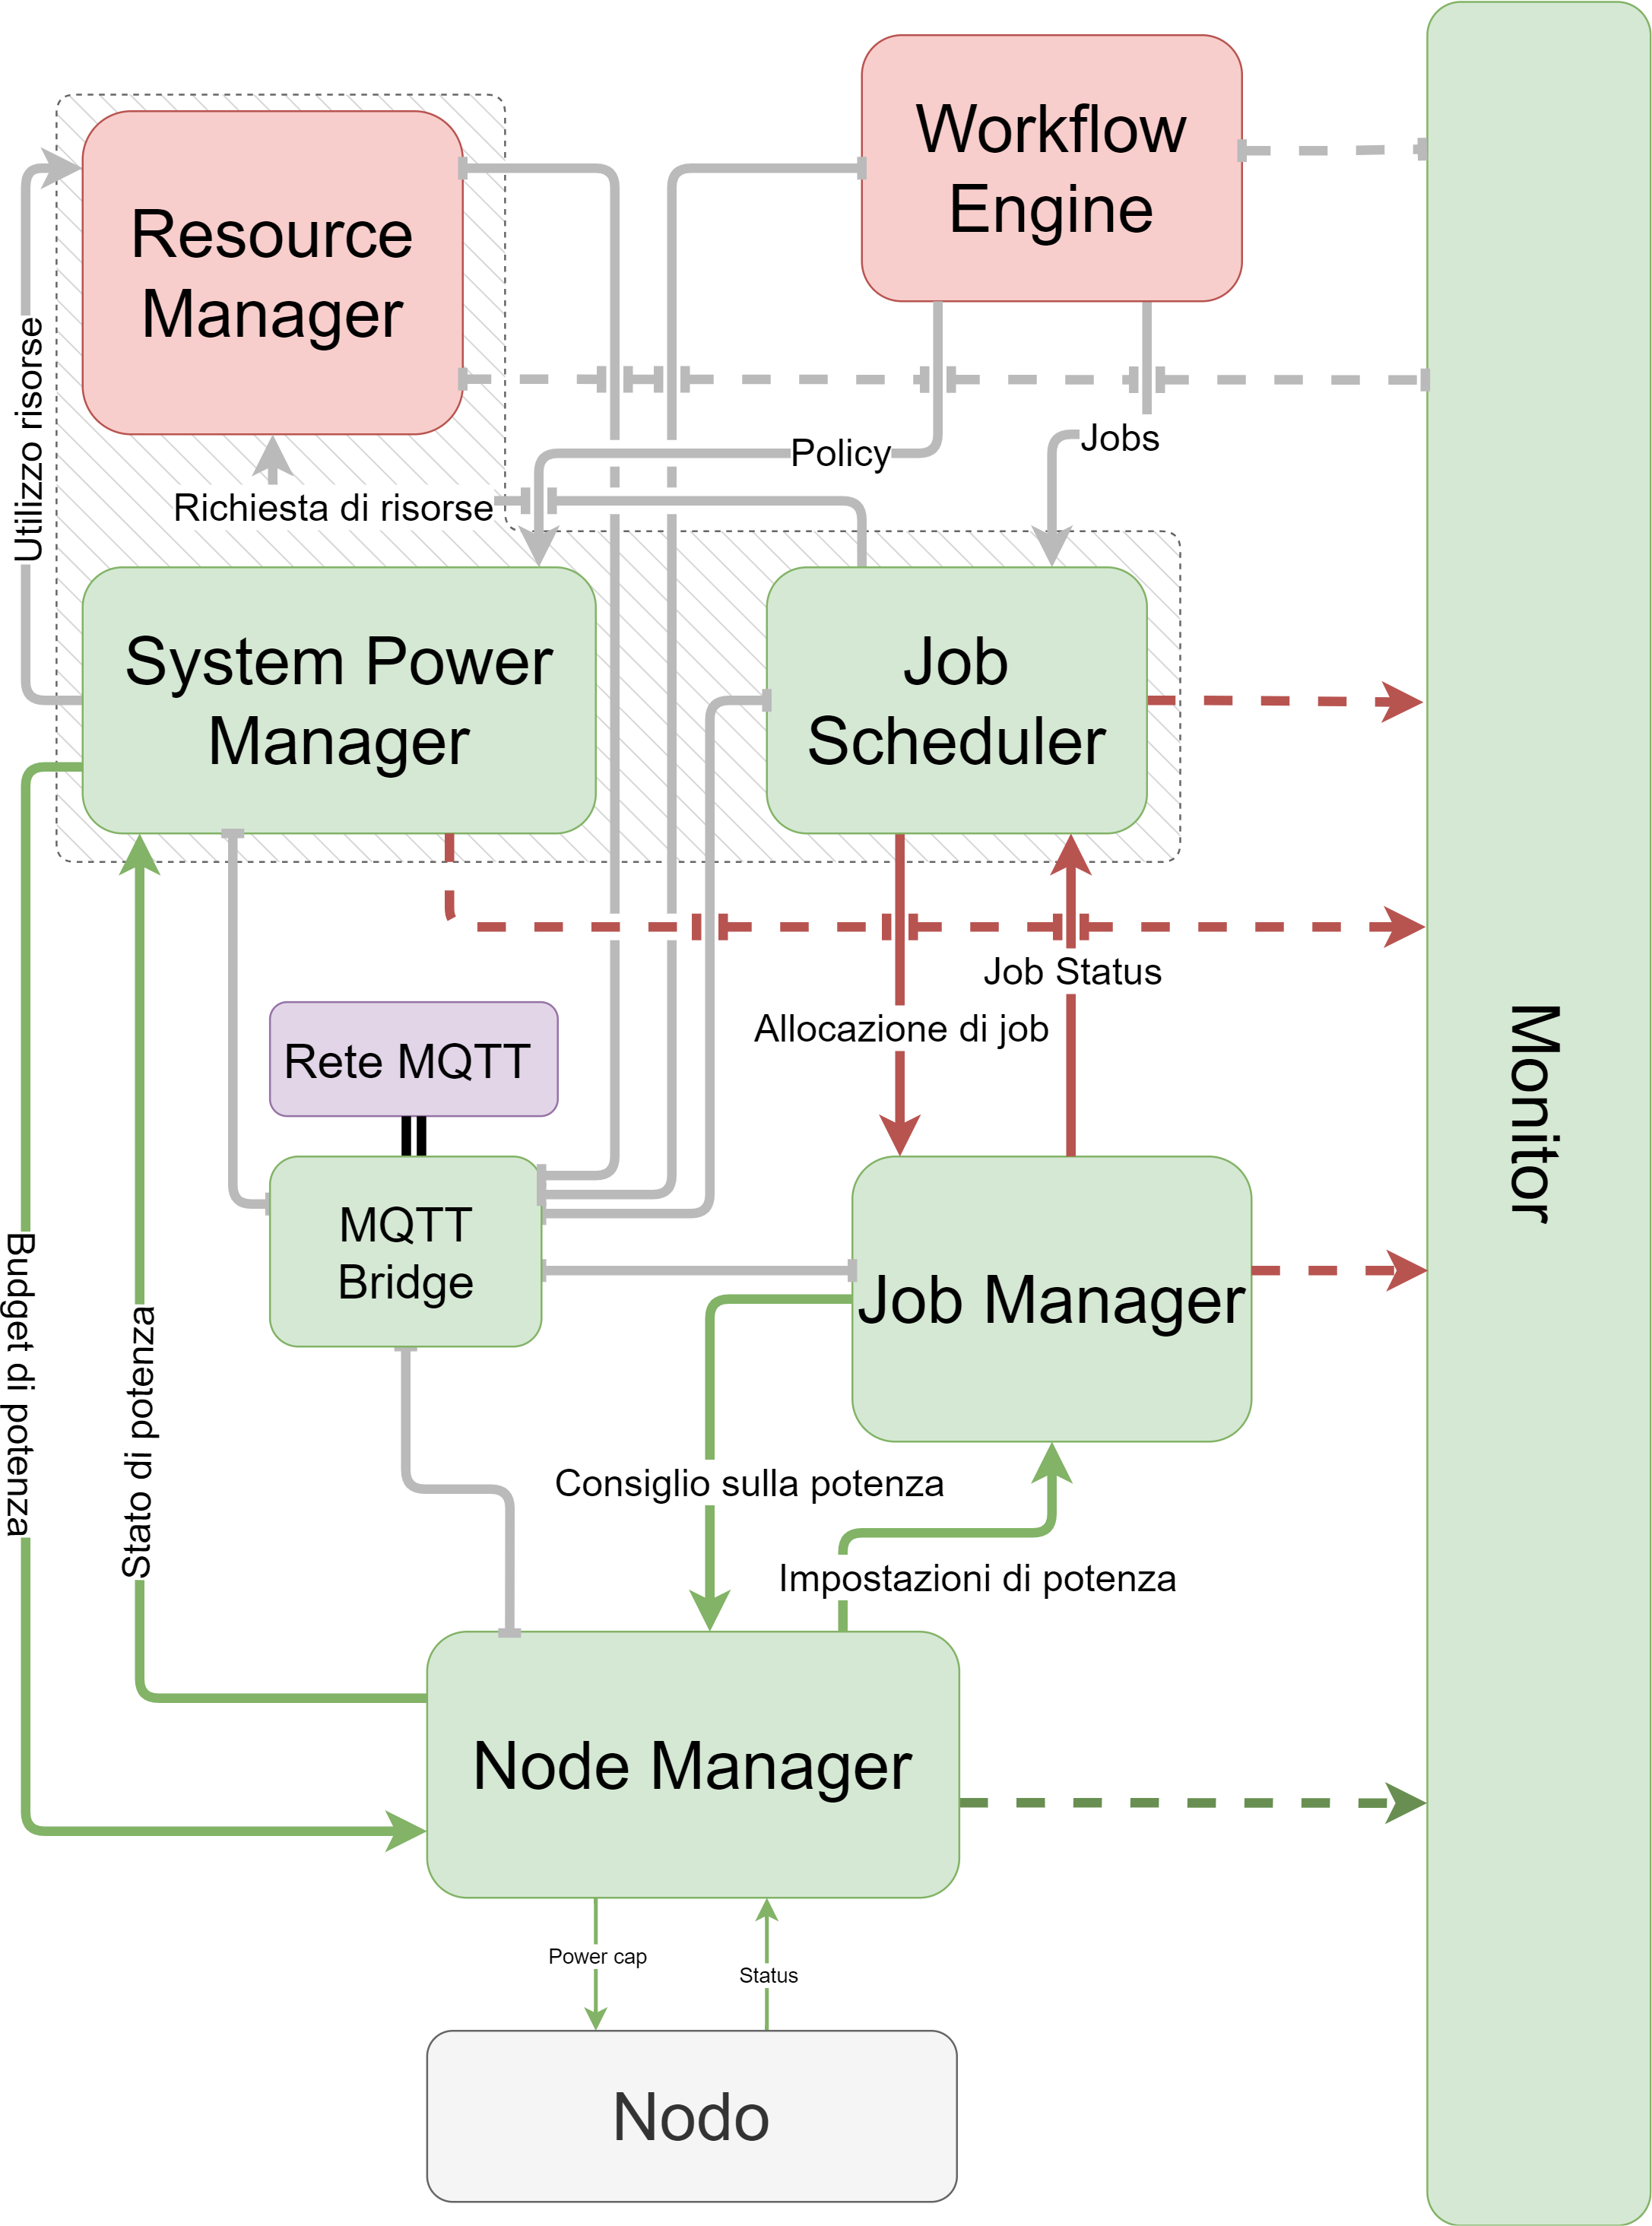
\includegraphics[width=\textwidth]{./img/SchemaPowerStack_perdummy.drawio.png}
    \caption{Schema componenti sviluppati: in verde completato, in grigio non previsto, in rosso ancora da sviluppare}
\end{figure}

Viene riportato lo scheletro dei componenti con i relativi topic usati al fine di dare una visione completa e aggiuntiva rispetto al modello precedentemente stilato  
\begin{figure}[H]
    \centering
    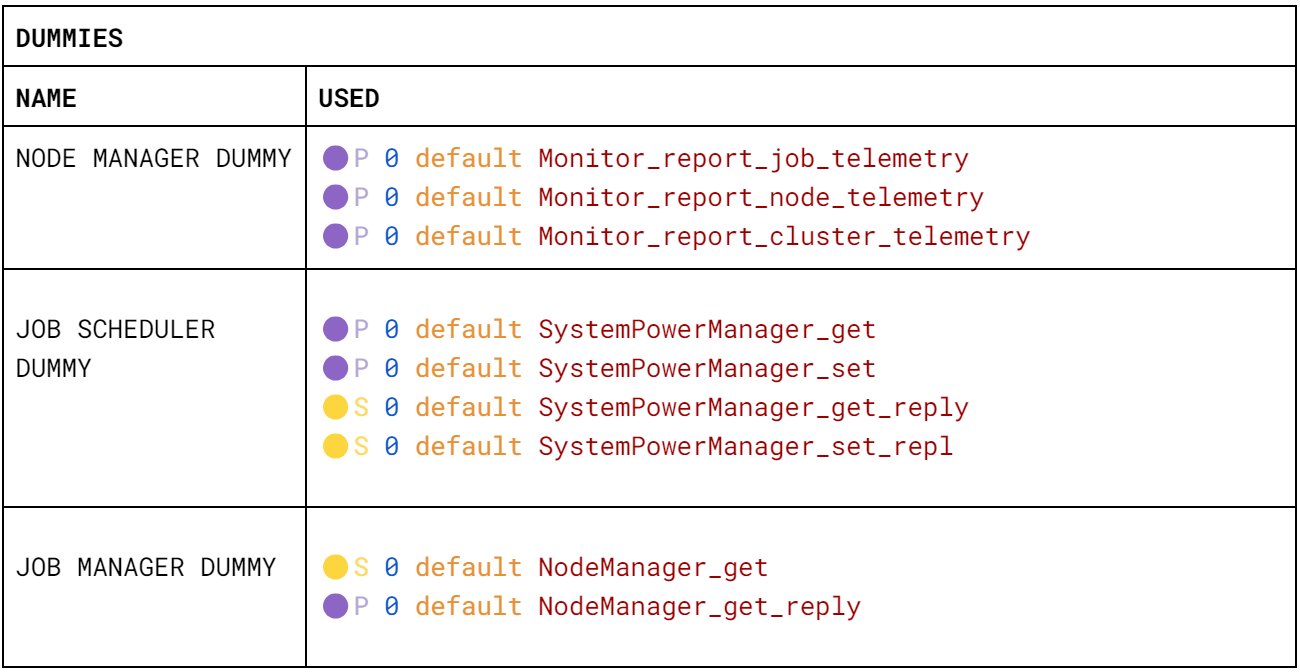
\includegraphics[width=\textwidth]{./img/dummies_skeleton.png}
    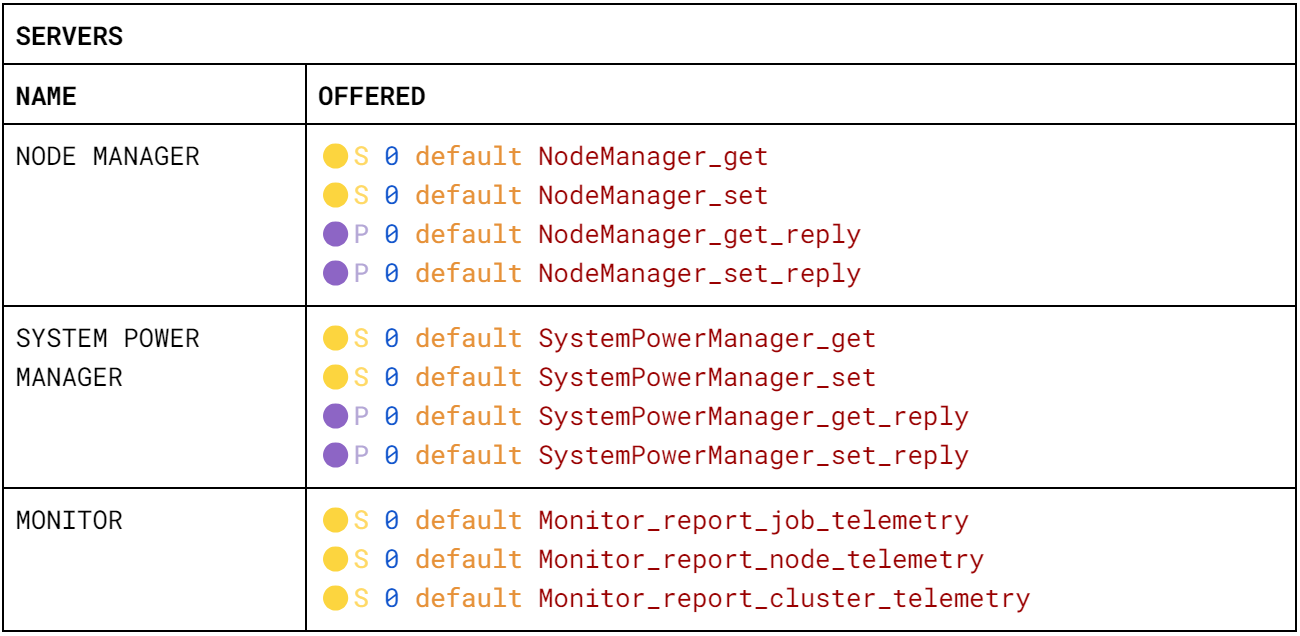
\includegraphics[width=\textwidth]{./img/server_skeleton.png}
\end{figure}